\documentclass[a4paper, 10pt, final]{article}
\usepackage{michael}

%% \def\mytitle{Signal and Image Processing 2010}
%% \def\mysubtitle{Handin of mandatory excercise 1}
%% \def\myauthor{Ulrik Bonde}
%% \def\mymail{\mailto{bonde@diku.dk}}
%% \def\mydate{\today}

\title{Signal and Image Processing 2010 \\ Mandatory hand-in exercise 1}
\author{Michael Andersen}
\date{\today}

%% \title{\mytitle}
%% \subtitle{\mysubtitle}

%% \author{\myauthor{} - \mymail}
%% \date{\mydate}

%% \hypersetup{
%% colorlinks,%
%% citecolor=black,%
%% filecolor=black,%
%% linkcolor=black,%
%% urlcolor=black,%
%% bookmarksopen=false,
%% pdftitle={\mytitle - \mysubtitle},
%% pdfauthor={\myauthor}
%% }

\begin{document}
\maketitle

\subsection*{Question 1.1}
We are to prove that Fourier transform of a real and even function is real and even.

\begin{equation*}
    \hat{g}(k) = \int_{-\infty}^{\infty}{g(x)\exp(-2\pi ikx)dx}
\end{equation*}
The above equation describes the 1-D Fourier Transformation, the equation is the same as eqn. 2.18 found on page 44 in the Digital Image Processing book.

The above equation can be split into two, and by changing the limits of the integral we change the sign. Lastly we substitute $x = -x$, thereby changing the sign in front of the second integral again.
\begin{align*}
    \hat{g}(k) & = \int_{-\infty}^{0}{g(x)\exp(-2\pi ikx)dx} + \int_{0}^{\infty}{g(x)\exp(-2\pi ikx)dx}\\
               & = \int_{0}^{\infty}{g(x)\exp(-2\pi ikx)dx} - \int_{0}^{-\infty}{g(x)\exp(-2\pi ikx)dx}\\
               & = \int_{0}^{\infty}{g(x)\exp(-2\pi ikx)dx} + \int_{0}^{\infty}{g(-x)\exp(2\pi ikx)dx}
\end{align*}

We now use the fact that we know that $g(x) = g(-x)$ because $g(x)$ is even, this results in the following equation:
\begin{equation*}
  = \int_{0}^{\infty}{g(x)\exp(-2\pi ikx)dx} + \int_{0}^{\infty}{g(x)\exp(2\pi ikx)dx}
\end{equation*}

By applying \textit{Euler's identities} $\cos(\theta) =
\frac{e^{i\theta} + e^{-i\theta}}{2}$. Setting $\theta = 2\pi kx$ and multiplying by $2$. We get the following:

\begin{align*}
  & = 2 \int_{0}^{\infty} {g(x) \frac{e^{i2\pi kx} + e^{-i2\pi kx}}{2}dx} \\
  & = 2 \int_{0}^{\infty}{g(x) \cos{(2\pi kx)}}
\end{align*}

The result $2 \int_{0}^{\infty}{g(x) \cos{(2\pi kx)}}$ only contains real parts, and therefore the result is real. We know that $g(x)$ is even, and the same applies to $\cos{(x)}$. This proves that the Fourier transform of a real and even function is also real and even.

\subsection*{Question 1.2}
We are to find the Fourier tranform of $\delta_{x,x_{0}} + \delta{x,-x_{0}}$. This is done as follows (calculation has been split into two integrals for ease)first part:
\begin{equation*}
   \int_{-\infty}^{\infty} {\delta_{x,x_{0}} e^{-2\pi ikx}dx}
\end{equation*}
\[
  = e^{-2 \pi ikx_{0}}
\]
This is because of the properties of the $\delta$-function which is only ``active'' when $x = x_{0}$. The other integral is almost symmetrical to the above, being:
\begin{equation*}
   \int_{-\infty}^{\infty} {\delta_{x,-x_{0}} e^{-2\pi ikx}dx}
\end{equation*}
\[
  = e^{2 \pi ikx_{0}}
\]
The combination of the above two equations are:
\[
e^{-2\pi ikx_{0}} + e^{2\pi ikx_{0}}
\]
Again we can apply \textit{Euler's identities}, as we are missing the denominator, we need to multiply the result by $2$
\[
= 2 \cos{(2\pi kx_{0})}
\]

We now need to show the Fourier transform of $\cos{(2\pi
  xu_{0})}$. Trying to integration of this would probably end
horribly. Instead perform a guess based on the above calculation, our
guess being $\frac{1}{2}(\delta_{x,u_{0}} +
\delta_{x,-u_{0}})$. Performing similar steps as above we get:
\begin{align*}
  \hat{g}(k) & = \frac{1}{2} \int_{-\infty}^{\infty} {(\delta_{x,u_{0}} +\delta_{x,-u_{0}})\exp{-2\pi ikx}dx}\\
  & = \frac{1}{2} 2 \cos{(2\pi ku_{0})} \\
  & = \cos{(2\pi ku_{0})}
\end{align*}
Therefore our guess was correct and the result is
$\frac{1}{2}(\delta_{x,u_{0}} + \delta_{x,-u_{0}})$

\subsection*{Question 1.3}
???
\subsection*{Question 1.4}
We are to write program that reads in an image and performs a reduction of the number of grayscale colors used in the image and modify/write another that is able to perform resolution reduction.

\begin{figure}[!h]
\centering
\subfloat[]{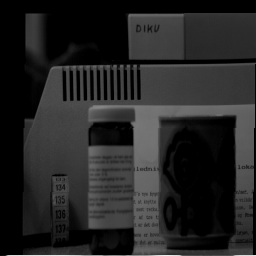
\includegraphics[width=0.3\textwidth]{images/img00}}
\subfloat[]{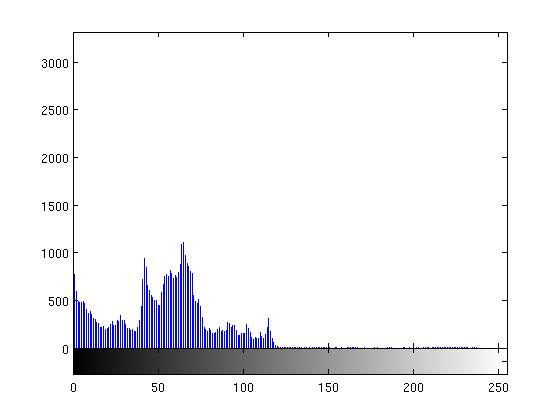
\includegraphics[width=0.5\textwidth]{images/img00h}}
\caption{Original image and histogram, unadjusted}
\label{fig:original}
\end{figure}
The figure \ref{fig:original} shows the original image and its histogram. It can be seen from the histogram that the image does not facilitate the entire gray colormap. Therefore I perform a image adjusting using the built-in \emph{imadjust} in MatLab to convert the picture to use the entire gray colormap, resulting in the image and histogram shown in \ref{fig:original_adjusted}. I will be working on the adjusted image for the remaining of this exercise. 

\begin{figure}[!h]
\centering
\subfloat[]{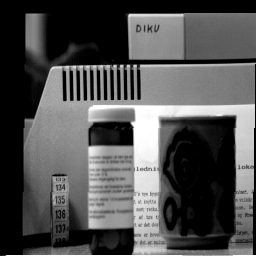
\includegraphics[width=0.3\textwidth]{images/img01}}
\subfloat[]{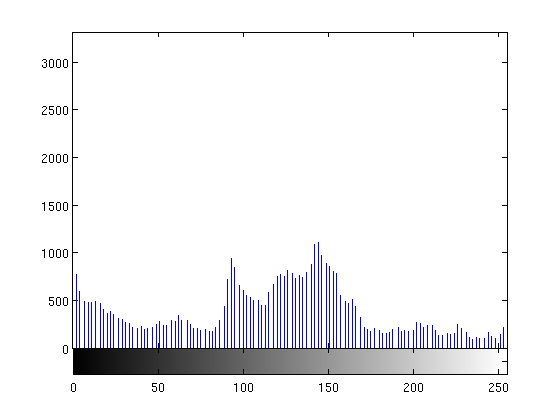
\includegraphics[width=0.5\textwidth]{images/img02}}
\caption{Original image and histogram, adjusted}
\label{fig:original_adjust}
\end{figure}

It is worth mentioning that without the adjustment of the images
colormap some troubles can arise when reducing the number of grayscale
colors. This is because the algorithm for reducing the colors rely on
the bins generated the built-in MatLab function
\emph{imhist}. Therefore, if the image colormap does not span the
entire colormap some of these bins will be empty, resulting in fewer
colors remaining than expected.

\begin{figure}[!h]
\centering
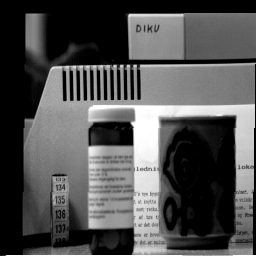
\includegraphics[width=1.0\textwidth]{images/img01}
\caption{Reduction range from 64--2 gray colors, adjusted}
\label{fig:reduceGray_range}
\end{figure}
The figure \ref{fig:reduceGray_range} show 

\begin{figure}[!h]
\centering
\subfloat[]{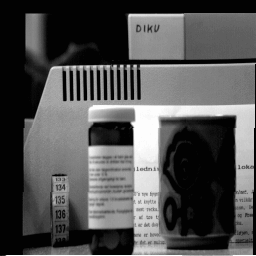
\includegraphics[width=0.3\textwidth]{images/img03}}
\subfloat[]{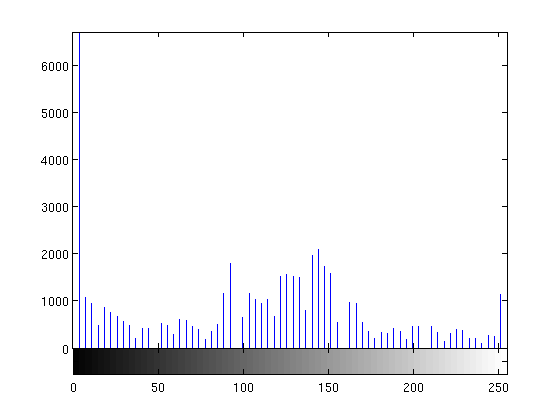
\includegraphics[width=0.5\textwidth]{images/img04}}
\caption{Reduced to 64 gray colors, image and histogram}
\label{fig:reduceGray64}
\end{figure}

\begin{figure}[!h]
\centering
\subfloat[]{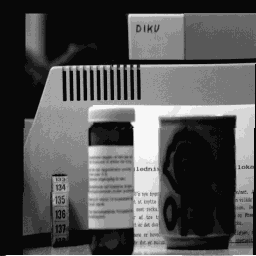
\includegraphics[width=0.3\textwidth]{images/img05}}
\subfloat[]{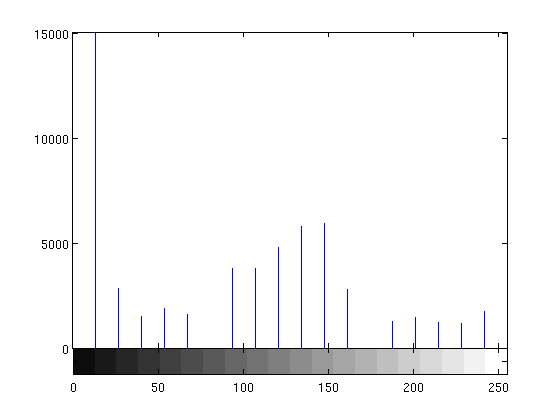
\includegraphics[width=0.5\textwidth]{images/img06}}
\caption{Reduced to 16 gray colors, image and histogram}
\label{fig:reduceGray16}
\end{figure}

\begin{figure}[!h]
\centering
\subfloat[]{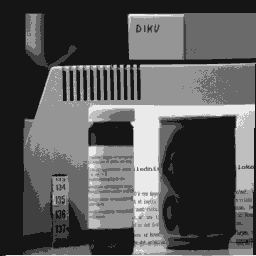
\includegraphics[width=0.3\textwidth]{images/img07}}
\subfloat[]{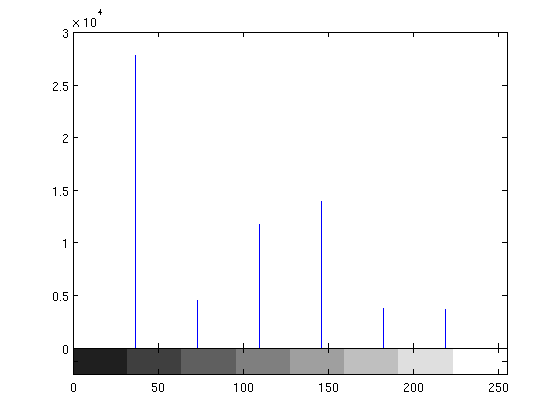
\includegraphics[width=0.5\textwidth]{images/img08}}
\caption{Reduced to 6 gray colors, image and histogram}
\label{fig:reduceGray6}
\end{figure}

\begin{figure}[!h]
\centering
\subfloat[]{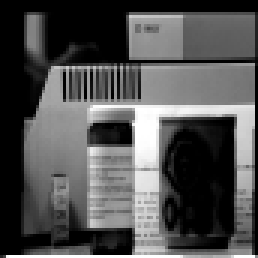
\includegraphics[width=0.3\textwidth]{images/img09}}
\subfloat[]{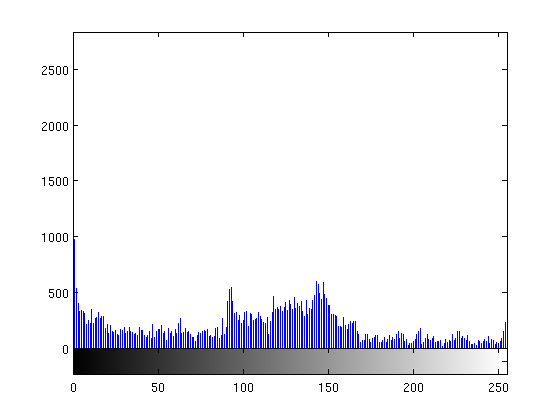
\includegraphics[width=0.5\textwidth]{images/img10}}
\caption{Resolution changed by factor 3, image and histogram}
\label{fig:resolutionFactor3}
\end{figure}

\begin{figure}[!h]
\centering
\subfloat[]{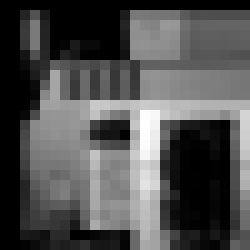
\includegraphics[width=0.35\textwidth]{images/img11}}
\subfloat[]{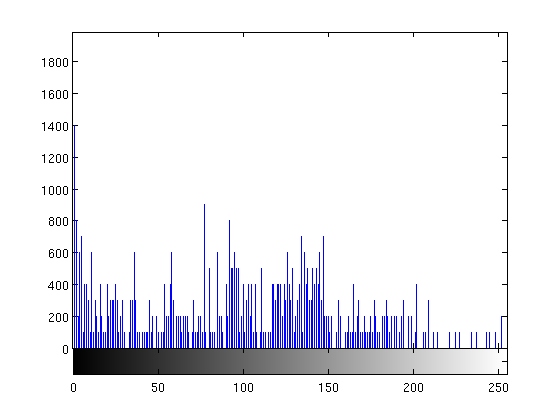
\includegraphics[width=0.5\textwidth]{images/img12}}
\caption{Resolution changed by factor 10, image and histogram}
\label{fig:resolutionFactor10}
\end{figure}


%%%%%%%%%%%%%%%%%%%%%%%%%%%%%%%%%%%%%%%%%%%%%%%%%%%%%%%%%%%%%%%%%%%%
% Formal stuff

\bibliographystyle{abbrvnat}
\bibliography{bibliography}
%\addcontentsline{toc}{chapter}{Litteratur}

\end{document}

% vim: set tw=72 spell spelllang=en:
